\chapter{Página principal y menú}
\label{cap:inicio}

\section{Página principal}

\captura{home}{Página principal}

Al ingresar se ve el saludo, la fecha y la hora del local. Quien tiene acceso a Caja ve además el \textbf{Resumen de hoy}, que se actualiza solo cada 30 segundos:

\begin{itemize}
  \item \textbf{Caja}: lo vendido y en cuántas ventas, lo cobrado en efectivo y por QR, y las mesas ocupadas con lo que falta cobrar.
  \item \textbf{Cocina}: los envíos en preparación, las unidades por preparar, los envíos listos para entregar y la espera más larga, con la mesa.
\end{itemize}

Más abajo están los \textbf{accesos rápidos} a las pantallas del cargo.

\section{Menú lateral}

El menú de la izquierda muestra solo las pantallas que su cargo puede ver. \pantalla{Administración} se despliega para mostrar sus pantallas. La pestaña redonda del borde contrae el menú para dejar solo los íconos, y el sistema recuerda cómo lo dejó.

\section{En celular y tablet}

\begin{figure}[H]
  \centering
  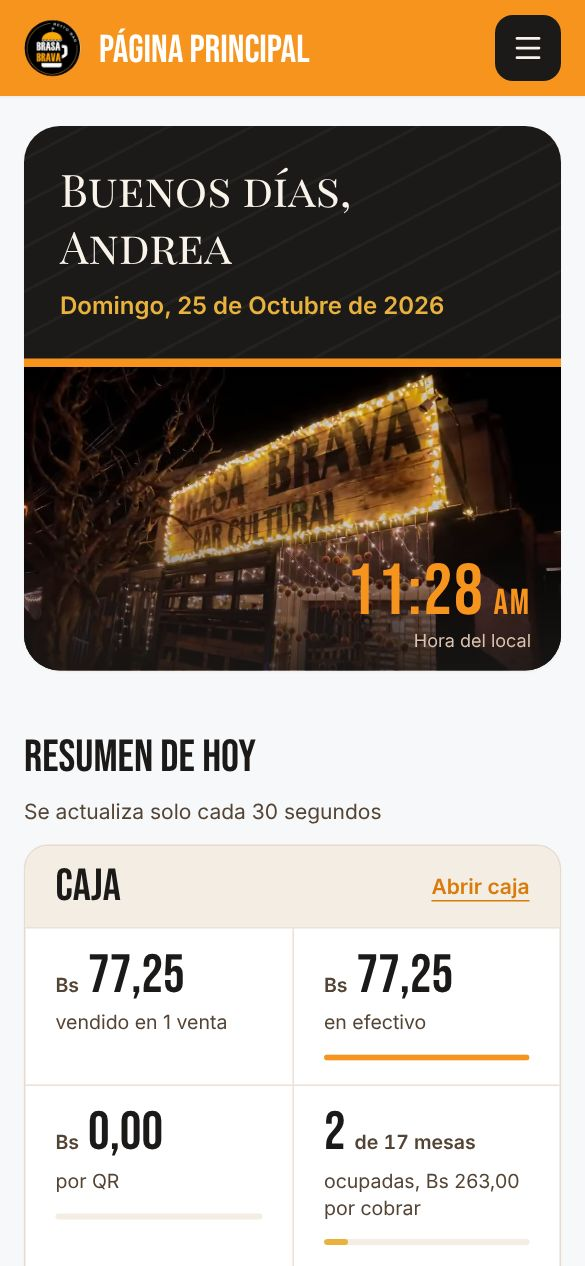
\includegraphics[width=0.3\linewidth]{celular-home}\hfill
  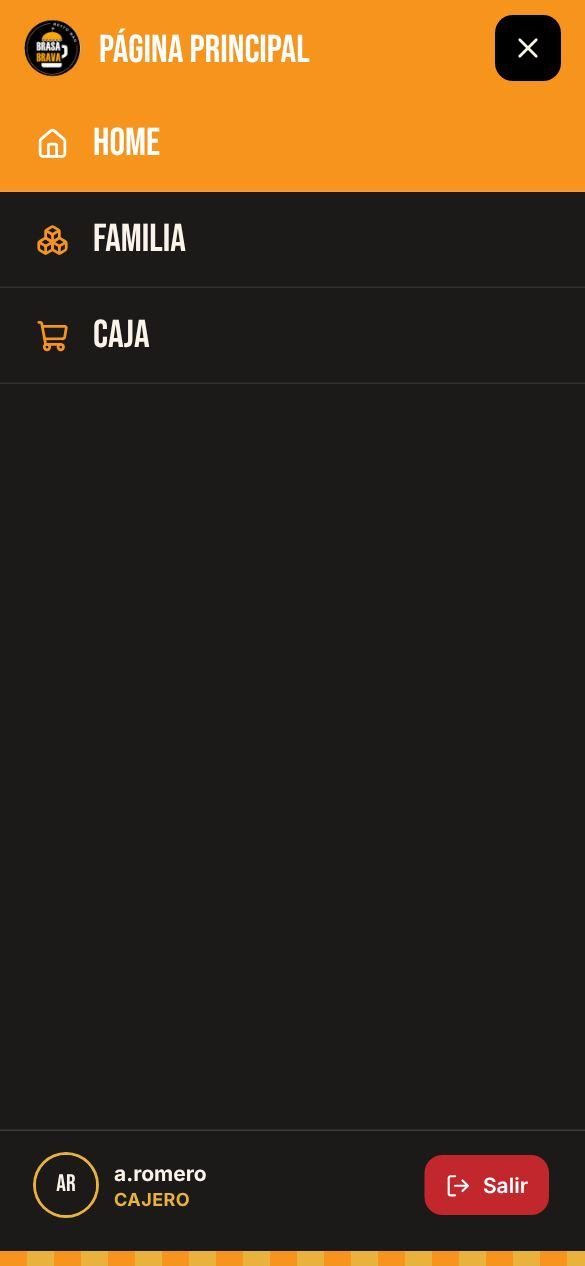
\includegraphics[width=0.3\linewidth]{celular-menu}\hfill
  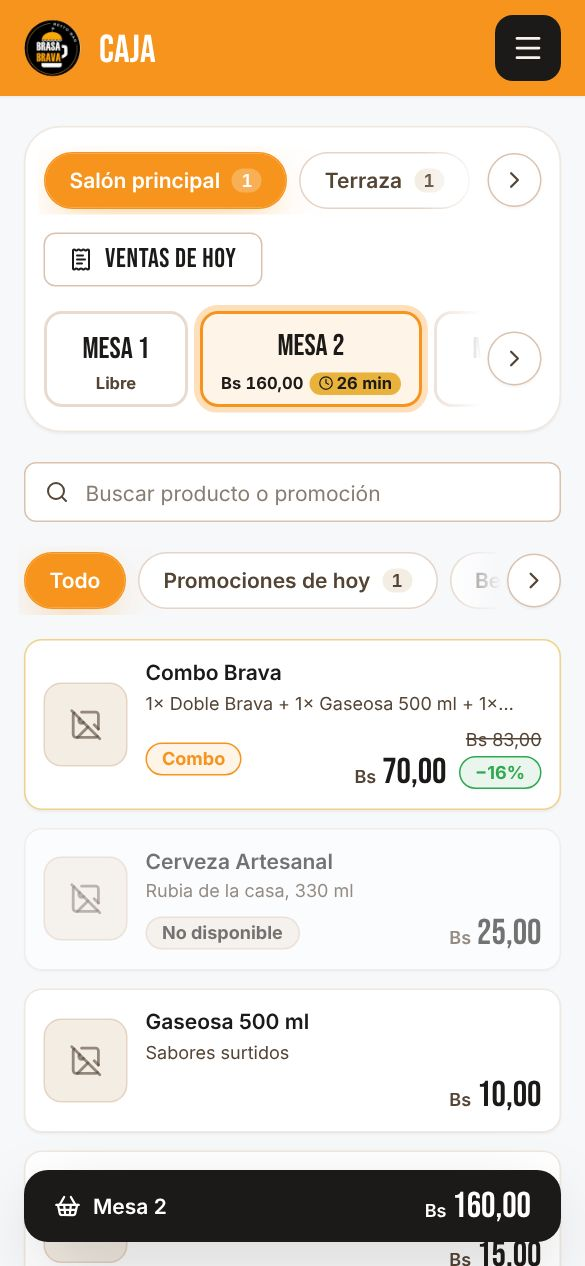
\includegraphics[width=0.3\linewidth]{celular-caja}
  \caption{Página principal, menú y Caja en el celular}
\end{figure}

En pantallas angostas el menú baja desde la barra naranja con el botón de la derecha y se cierra con la X, con la tecla Escape o al elegir una pantalla. Las tablas se muestran como tarjetas. En Caja, el pedido de la mesa se abre desde la barra inferior.
